\documentclass{article}
\usepackage[margin=1in]{geometry}
\usepackage{graphicx}
\usepackage{subfig}
\usepackage{amsmath}

\newcommand{\ie}{ \textit{i.e} }

% Author information
\author{Thomas Binu}
\title{\textbf{A Study on Multi-Object Motion Tracking\\Computer Vision Project Report}}

\begin{document}
	\maketitle
	\section{Introduction}
	The goal of this project is to track and analyze moving traffic from a video footage. We will examine some computer vision based techniques for multi-object motion tracking and simulate a working sample using MATLAB. Motion tracking and speed estimation through computer vision have numerous application in the industry in the areas of Autonomous Vehicle Systems, Traffic Control, Geographical Information Systems, Motion Blur Reduction etc.
	
	\subsection{Defining the problem}
	The project can be broken down into the two parts
	\begin{enumerate}
		\item Identifying moving vehicles from the background \ie the foreground object detection.
		\item Tracking and predicting the motion of vehicles \ie object tracking	
	\end{enumerate}
	
	\subsection{Foreground object detection}
	Since the objective is to track moving vehicles from a video,we can rule out approaches based on segmenting foreground objects from still images, and turn our focus to detecting relative motion of objects between different images. This way, our solution become applicable to moving objects of any shape or size or color.
	
	The first step is to identify foreground objects in the given video. This technique is called \textit{background subtraction} and is commonly used in traffic monitoring, objecting tracking and advanced human interfaces. A flexible and reliable method of background subtraction should handle 
	
		\begin{enumerate}
		\item Subtle illumination changes to the background because of lighting conditions.
		\item Noise or minute high-frequency repetitive motions such as movement of leaves, grass, dust etc.
		\end{enumerate}
	
	\subsubsection{Naive Approach}
	A rough estimation of the foreground objects can be made by using simple \textit{frame differencing} ie taking the difference between two consecutive frames with a threshold. Depending on the value of the threshold used and frame differences, the quality of the results will differ but in general, this approach is erratic and unreliable. 
	
	This approach can be further refined by using a mean or median of the previous n frames to estimate the background and construct a foreground mask by taking the difference of the background and the current frame. 
	
	\begin{figure}
		\centering
		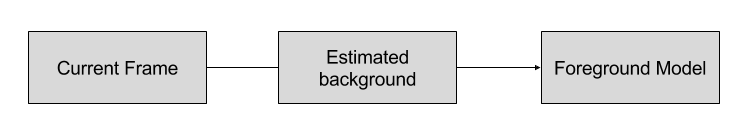
\includegraphics[scale = 0.4]{figures/naive_fd.png}
		\caption{Foreground estimation using frame differencing}
	\end{figure}
	
	\subsubsection{Background Subtraction using Gaussian Mixture Model}
	 
	This approach based on a paper by Chris Stauffer and W.E.L Grimson discusses using a mixture of adaptive \textit{Gaussian for background subtraction} By using a set of training frames, a multivariate Gaussian Mixture probabilistic model is then created for the background pixels. That pixels which do not match with the model is classified as a foreground pixel.
	
	Advantages of Background subtraction using GMM
	
	\begin{enumerate}
		\item There is a different threshold for each pixel based based on its location and training set of frames
		\item The pixel wise threshold is adapted over time.
		\item This model can handle gradual variations in lighting conditions and high-frequency noise.
	\end{enumerate}

	\begin{figure}[!h]
		\centering
		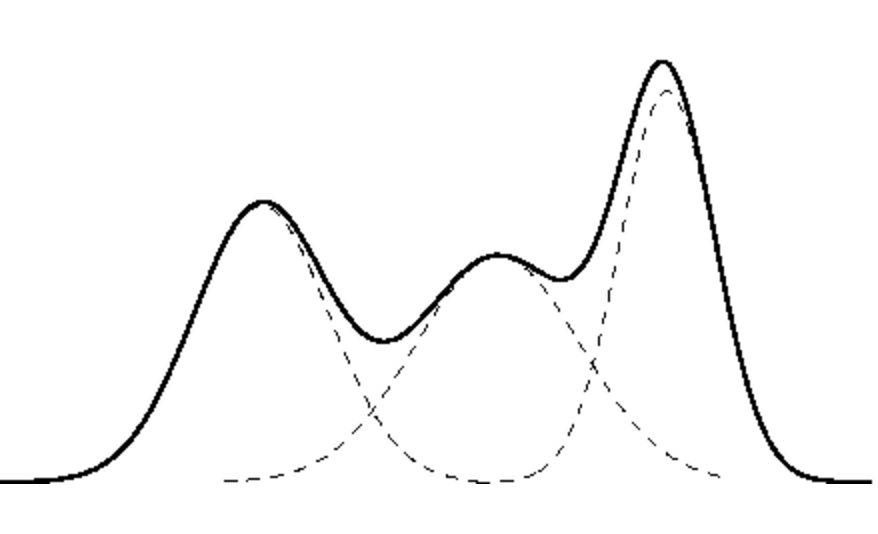
\includegraphics[scale = 0.3]{figures/gmm_graph.png}
		\caption{Gaussian mixture models (GMM)}
	\end{figure}

	\subsection{Motion Tracking}
	
	\subsubsection{Noise removal}
	After you perform background subtraction on the input video, the foreground binary image is run through a preprocessing step called \textit{morphological opening} to remove the excess salt and pepper noise. This process involves sliding a small shape or template called the structuring element over the image. The structuring element is placed at all possible active pixels over the image and compared with the neighboring pixels, and the center pixel is either set to 0 or 1 depending on the operation. Morphological opening is erosion followed by dilation, and is denoted by 
	\begin{align*}
		 A \circ B &= (A \ominus B) \oplus B \\ \text{where}& \ominus \text{ is erosion}, \oplus \text{ is dilation}
	\end{align*}
	
	\subsubsection{Blob Analysis}
	The foreground detector step will yield a binary image with multiple foreground objects. The next step will be to identify and track the objects between frames. Separating the foreground objects from the image and classifying and computing its various properties is called \textit{Blob Analysis}. Various algorithms exist for Blob Analysis. Given below are two common approaches
	
	\begin{enumerate}
		\item \textit{Grass-Fire Algorithm}: The algorithm scans the image from top right to bottom left. If it finds a foreground pixel(with a value of 1) it will be marked as 'visited' and added as a part of a blob object. Next, taking this pixel as the center, the algorithm checks the  neighboring pixels to see if any of them are also a foreground pixel. If yes, those pixels are added to the current blob object and marked as 'visited'. Then this visited pixel is taken as the center, and its neighbors are checked as described earlier. After all the pixels in the foreground object are added the the blob object, the algorithm moves through the image until the next foreground pixel is identified, which is taken as the second blob object. This process continues until all blobs are segmented.
		
		\item \textit{Laplacian of Gaussian}: One of the most common approaches for blob detection is based on the Laplacian of Gaussian(LoG). The basic algorithm is as follows
		
		\begin{enumerate}
			\item Filter the image with Gaussian at different scales
			\item Find the difference in the images from above to approximate the Laplacian			
			\item  Thus, it will yield maximal responses if applied to an
			image neighborhood that contains a similar  blob structure at
			a corresponding scale. By searching for scale-space extrema of the LoG, we can
			therefore detect circular blob structures.
		\end{enumerate}
	
	\begin{figure}[!h]
		\centering
		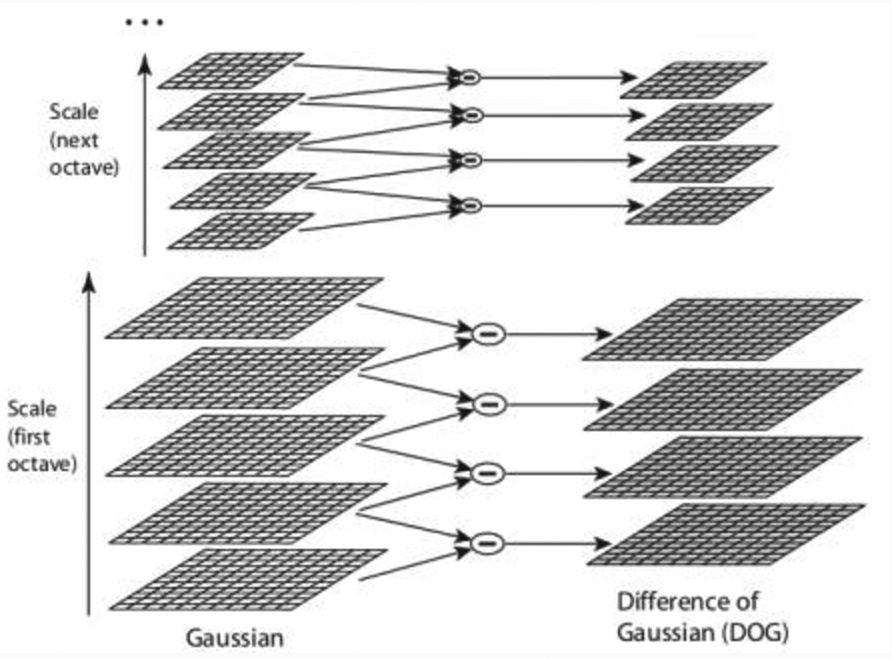
\includegraphics[scale = 0.4]{figures/DoG.png}
		\caption{Difference of Gaussian}
	\end{figure}
		
		
	\end{enumerate}
	
	\subsection{Kalman Filter}
	
	Kalman Filter, based of the seminal paper published in the 1960s, is an algorithm that uses a series of measurements over time to calculate the next measurement. Kalman Filter has a variety of application in the industry, especially in the field of navigation control and guidance. The algorithm can run in real time, with the only input being the current measurement and previously calculated state and uncertainty matrix, with no additional data required.
	
	When applied to motion estimation, Kalman filter will try to calculate the position of the moving object based on measurements of a set of previous positions. If the position measurements of the moving vehicle stop getting updated, for example if the vehicle is obstructed by another large vehicle the Kalman filter will try to predict the current position of the vehicle based on the variations and patterns calculated from the previous measurements.
	
	\begin{figure}[!h]
		\centering
		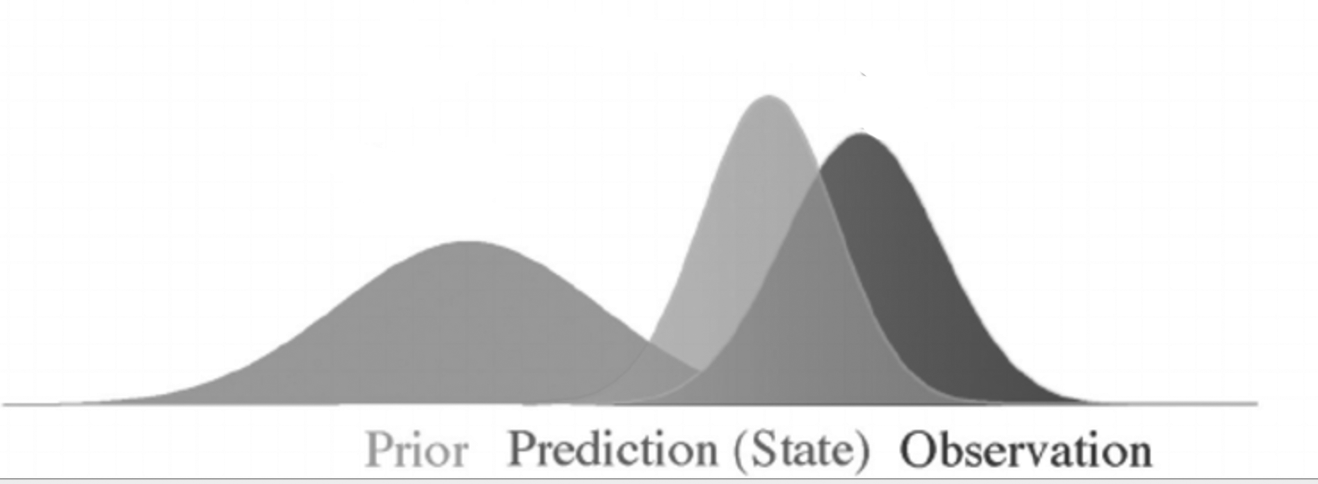
\includegraphics[scale = 0.4]{figures/kf_diagram.png}
		\caption{Kalman filter basic workflow}
	\end{figure}
	
	\section{Implementation}
	
	\subsection{Key Matlab Functions}
	Given below is a list of Matlab functions that was used in this project.
	
	\begin{enumerate}
		\item System Objects: Special MATLAB objects designed to handle streaming data efficiently. They have a step function to process streaming data and run the system object.
		
		\item Foreground Detector: Computer a foreground mask based on a series of training frames.
		
		\item imopen: To perform morphological opening. This method is used to remove salt and pepper noise from the output of Foreground detector.
	
		\item Blob Analysis: To perform connected component analysis in a binary image. This method will be used in the implementation to compute the bounding box of foreground objects.
		
	\end{enumerate}

	\subsection{Algorithm}

\begin{enumerate}
	\item Read the video file using vision.VideoReader System Object.
	
	\item Instantiate the foreground detector system object. A value of 50-100 for training frames works well for the example
	
	\item Instantiate the blob analysis detector. A value of 150 for minimum blob area works well for removing noise. 
	
	\item Train the foreground detector by running through the first 100 frames in the video.
	
	\item While loop through the video frame-by-frame
	
	\begin{enumerate}
		\item Calculate the foreground by using foreground detector.
		\item Clean up the foreground image using morphological opening.
		\item Calculate the bounding box of the blobs in the image using blob analysis
		\item Using the bounding box to draw a rectangle over the foreground images.
	\end{enumerate}

	\begin{figure}[!h]
		\centering
		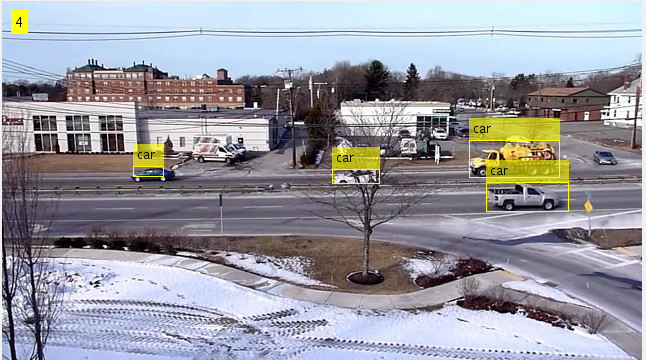
\includegraphics[scale = 1.0]{figures/output.png}
		\caption{A single frame from the output video}
	\end{figure}
	
\end{enumerate}
	\pagebreak
	\begin{thebibliography}{4}
		\bibitem{kalman} https://www.cs.unc.edu/~welch/kalman/media/pdf/Kalman1960.pdf 
		
		\bibitem{log}https://www.ncbi.nlm.nih.gov/pubmed/23757570
		
		\bibitem{gmm} http://www.isprs.org/proceedings/XXXVIII/part3/a/pdf/61\_XXXVIII-part3A.pdf
		
		\bibitem{matlab}https://www.mathworks.com/help/vision/examples/motion-based-multiple-object-tracking.html
		
		\bibitem{kalman-2} http://www.cs.unc.edu/~tracker/media/pdf/SIGGRAPH2001\_CoursePack\_08.pdf	
	\end{thebibliography}
	
\end{document}